\documentclass[a4paper,12pt]{article} 

%%% Работа с русским языком
\usepackage{cmap}                           % поиск в PDF
\usepackage{mathtext} 			 	       % русские буквы в формулах
\usepackage[T2A]{fontenc}               % кодировка
\usepackage[utf8]{inputenc}              % кодировка исходного текста
\usepackage[english,russian]{babel}  % локализация и переносы
\usepackage[left=2cm,right=2cm,
    top=2cm,bottom=3cm,bindingoffset=0cm]{geometry}
\usepackage{wrapfig}
\usepackage{gensymb}
\usepackage{textcomp}
\usepackage{multirow}
\usepackage{pgfplots}
\usepackage{amsmath,amsfonts,amssymb,amsthm,mathtools} % AMS
\usepackage{euscript}	 % Шрифт Евклид
\usepackage{mathrsfs} % Красивый матшрифт
\usepackage{graphicx}%Вставка картинок правильная
\usepackage{float}%"Плавающие" картинки
\usepackage{wrapfig}%Обтекание фигур (таблиц, картинок и прочего)
\title{Лабораторная работа 7.4

Изучение поглощения космического излучения в свинце}
\author{Кагарманов Радмир Б01-102}
\date{23 октября 2023 г.}

\begin{document}
\maketitle
\thispagestyle{empty}
\newpage
\setcounter{page}{1}

\paragraph{Цель работы:} измерить зависимость космического излучения от толщины поглотителей.

\paragraph{В работе используется:} космический телескоп, блок управления и индикации(БУИ).

\paragraph{Теория\\}
Космические лучи - это заполняющие все космическое пространство микрочастицы с высокой энергией, называемые также первичным космическим излучением.
Они состоят в основном из протонов и $\alpha$-частиц.\par
Вторичное космическое излучение возникает вследствие прохождения космических лучей через атмосферу. Оно состоит из следующих компонент.
\subparagraph{1.} адронная компонента, взаимодействующая с ядрами элементов, состоит из нуклонов и мезонов.
\subparagraph{2.} жёсткая компонента, которая генерируется в результате распада заряженных пионов.
\subparagraph{3.} мягкая компонента, возникающая из-за распада нейтральных пионов с образованием квантов высокой энергии.\\ \par
В эксперименте измеряется зависимость интенсивности космического излучения от толщины свинцовых пластин. С потерей энергии частицей уменьшается интенсивность вторичного космического излучения, которое ослабляется за счёт сильновзаимодействующих частиц мягкой компоненты, практически полностью поглощаемой свинцовыми пластинами. Это позволяет измерить отношение интенсивностей жёсткой компоненты, имеющей большую проникающую способность, к суммарной интенсивности в отсутствии пластин.

\paragraph{Установка\\}
Основой измерительной установки является телескоп, отбирающий для регистрации лишь те частицы, которые проходят в определённом направлении. "Космический телескоп" состоит из нескольких рядов параллельно включенных счётчиков Гейгера - Мюллера. Он позволяет регистрировать только частицы, пролетевшие через все счётчики, что достигается с помощью схемы совпадений.\par
Схема КТ может поворачиваться вокруг оси крепления его к стойке на угол $\theta$, считываемый на круговом лимбе прибора.
БУИ установки содержит:
\subparagraph{1.} Таймер с максимальным временем измерения 999 с.
\subparagraph{2.} Схема совпадений.
\subparagraph{3.} Блок пересчёта импульсов.
\subparagraph{4.} Высоковольтный выпрямитель для питания счётчиков.
\begin{figure}[!h]
\centering
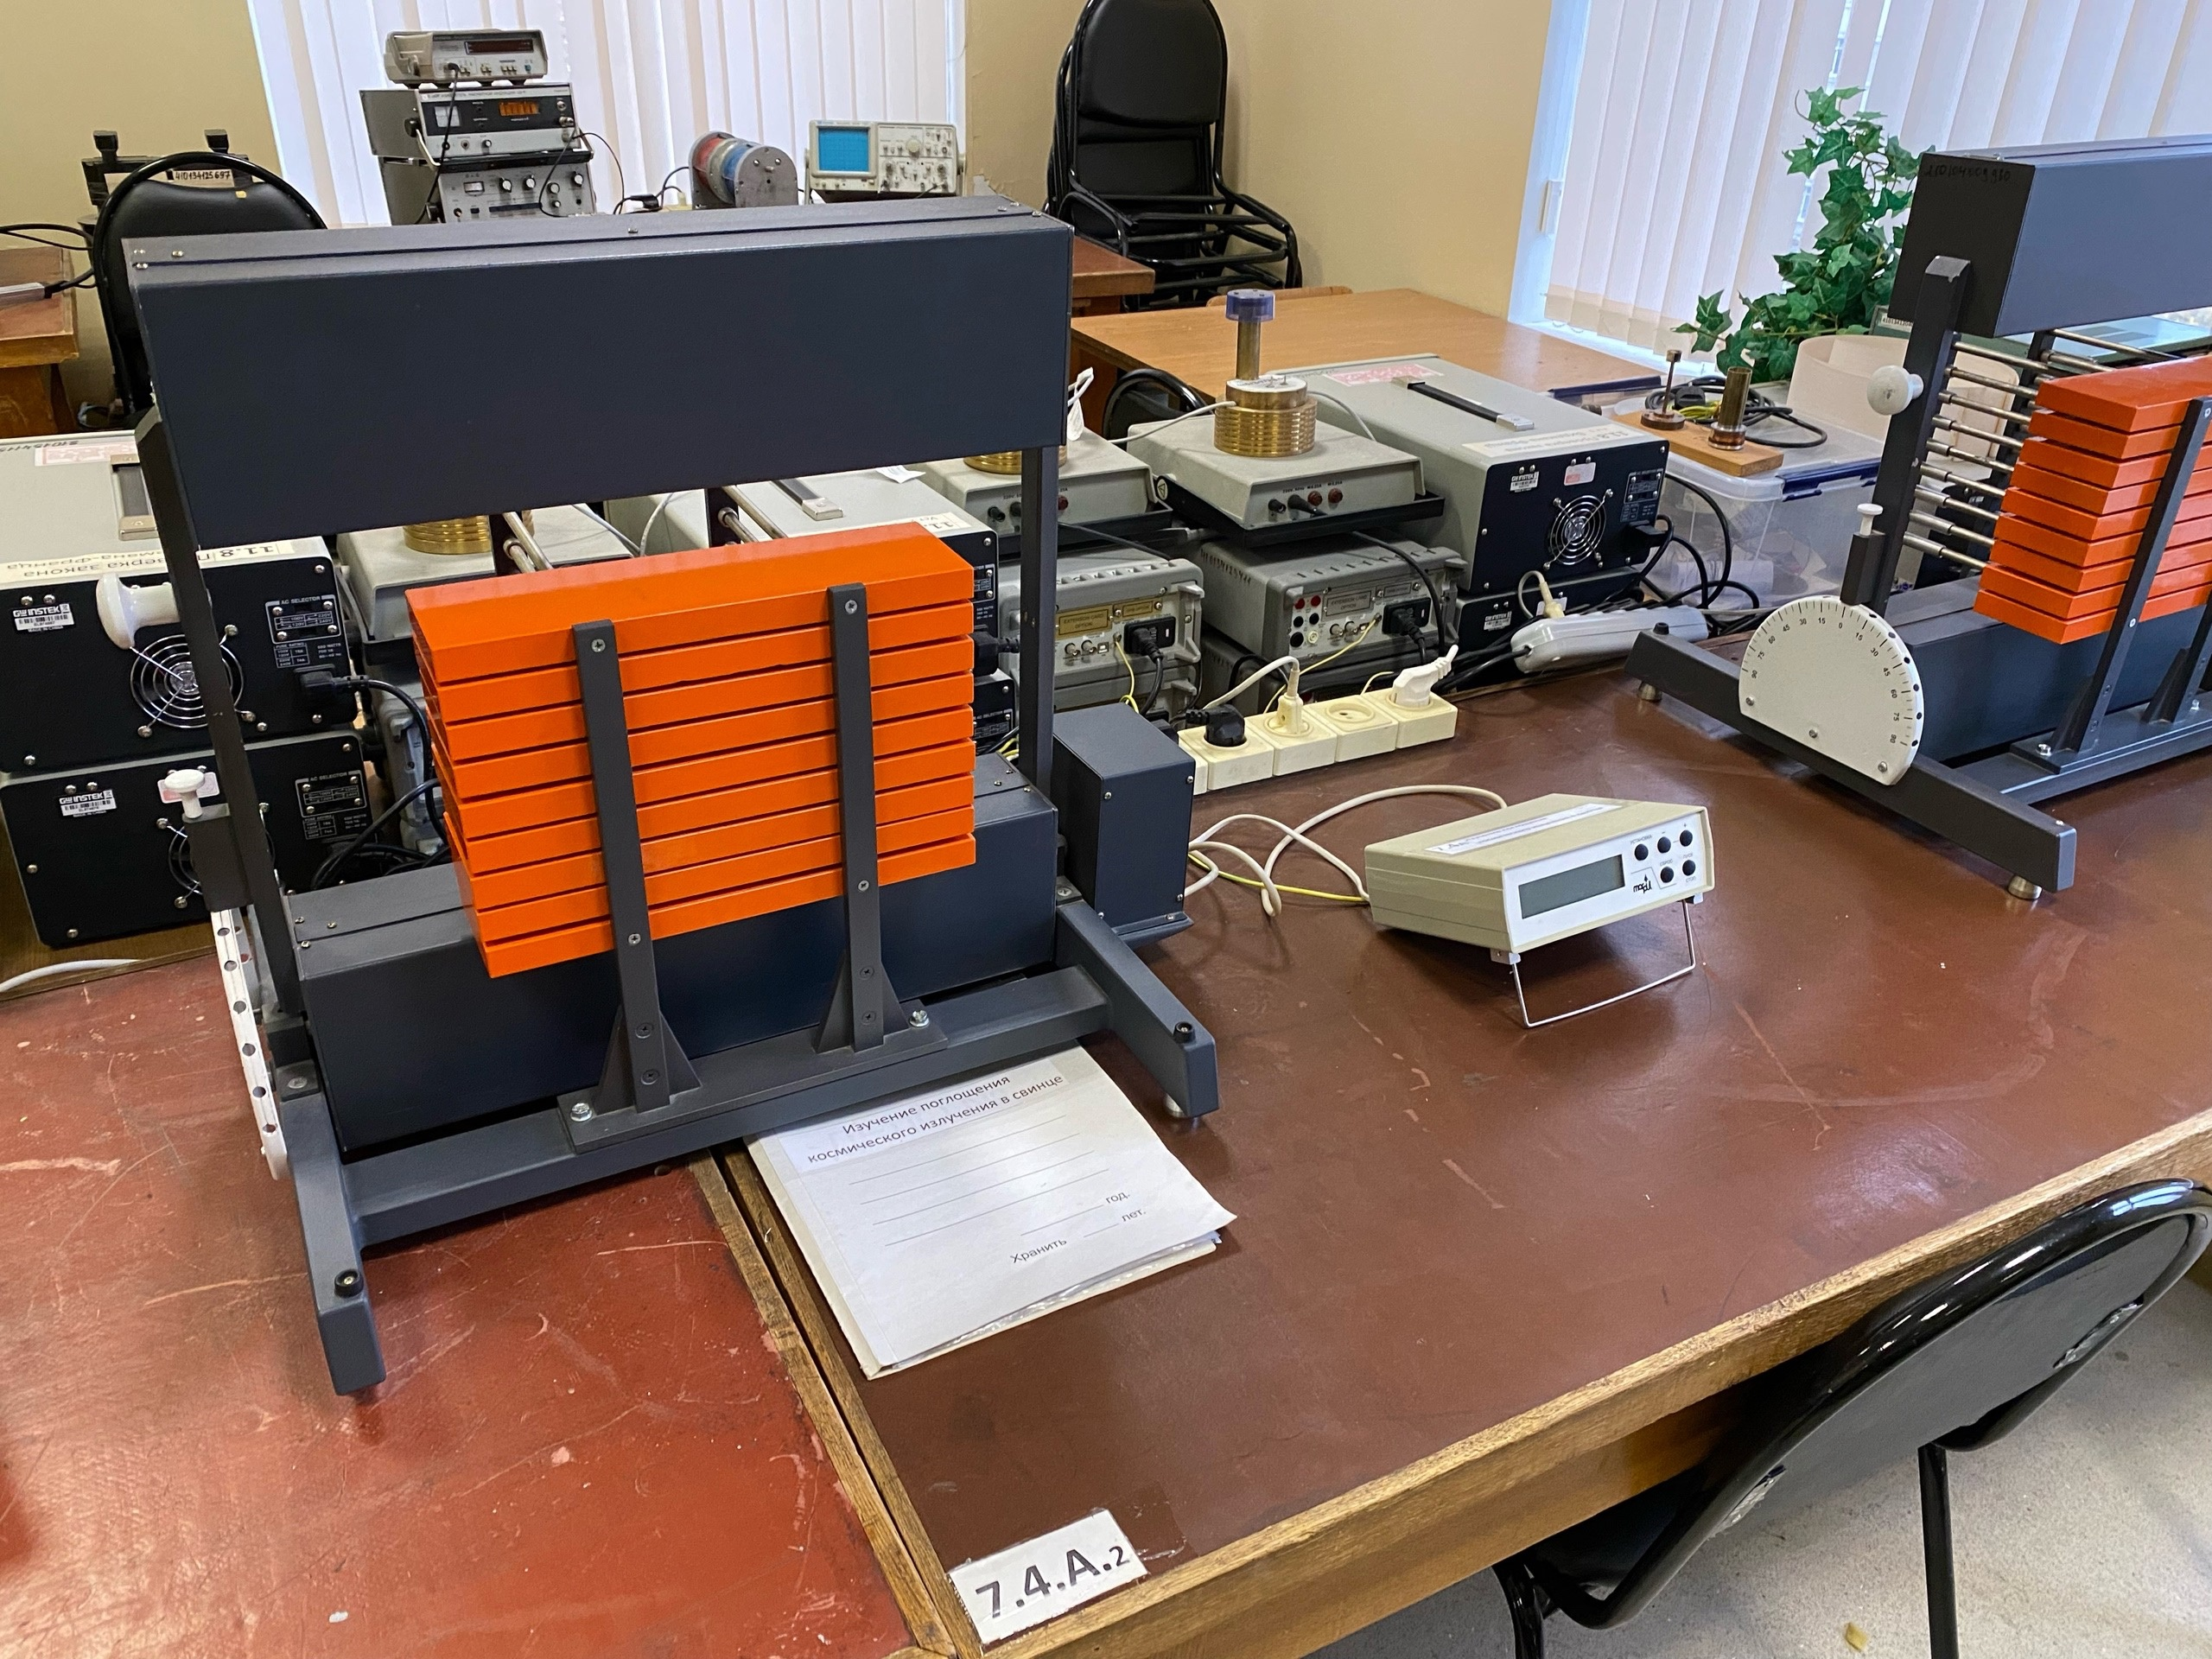
\includegraphics[width=0.8\linewidth]{mMjaFSDtkzc.jpg}
\caption{Экспериментальная установка}
\label{fig:mpr}
\end{figure}

\paragraph{Обработка результатов\\}
\subparagraph{1.} Мы измерили зависимость интенсивности излучения от увеличения количества пластин. В каждом эксперименте мы добавляли одну пластину. На Рис 2. представлен график. Результат не сошёлся с теорией. Это произошло из-за большой погрешности. Эксперименты нужно проводить дольше по времени. Если подставить измерения в формулу 
\begin{equation}
    \frac{I_{м}}{I_{ж}}=\frac{N_{i(d=0)}-N_{i(d=max)}}{N_{i(d=max)}},
\end{equation}
то получим, что $\frac{I_{м}}{I_{ж}}$=0,07.
\paragraph{2.} На Рис. 3 приведён график зависимости импульсов от угла наклона установки.
\begin{figure}[!h]
\centering

\includegraphics[width=1\linewidth]{graph1.png}
\caption{Зависимость интенсивности излучения от количества пластин}
\label{fig:mpr}
\end{figure}
\begin{figure}[!h]
\centering

\includegraphics[width=1\linewidth]{graph2.png}
\caption{Pависимость импульсов от угла наклона установки}
\label{fig:mpr}
\end{figure}

\paragraph{Вывод:} в данной лабораторной работе мы измерили зависимость интенсивности излучения от толщины поглотителя и от угла наклона установки. Результаты получились плохими, так как времени на эксперименты было немного, и из-за малого количества измеренных импульсов была большая погрешность.

\end{document}
